\documentclass{article}
\usepackage{amsmath}
\usepackage[pdftex]{graphicx}
\usepackage{subfigure}
\usepackage{indentfirst}

\title{Information Theoretic Modeling -- Exercise 3}
%\author{Haibo Jin}
\date{}


\bibliographystyle{plain}

\begin{document}

\maketitle

{\centering \large \textbf{Haibo Jin}}

{\centering \large \textbf{Student number: 014343698}}

\section{Problem 1}

\subsection*{(a)}

Based on Kraft inequality and Kraft-McMillan theorem, we can get the following:

SET1 should be the set of prefix(-free) codes.

SET2 should be the set of decodable codes.

SET3 should be the set of codes that satisfy the Kraft inequality.

SET4 should be the set of all possible symbol codes.


\subsection*{(b)}

For SET1 ${\subseteq}$ SET2, a code such as \textbf{$\{0, 01, 011, 0111\}$} satisfies, because it is decodable but not prefix(-free).   

For SET2 ${\subseteq}$ SET3, a code such as \textbf{$\{1, 10, 11\}$} satisfies, because it satisfies Kraft inequality but not decodable. 

For SET3 ${\subseteq}$ SET4, a code such as \textbf{$\{0, 1, 00\}$} satisfies, because it is just a symbol code but not satisfy Kraft inequality. 

\section{Problem 2}

The Shannon-Fano code is simulated by a program implemented in python, please refer to \emph{shannon\_fano.py} for more details.

Based on the result of the program, the expected code-length is \textbf{1.22}, the entropy is \textbf{0.683} and the expected code-length of the Shannon code is \textbf{1.5}. Figure 1 shows the running result of the program.

\vspace{5mm}
\begin{minipage}{0.9\textwidth}
  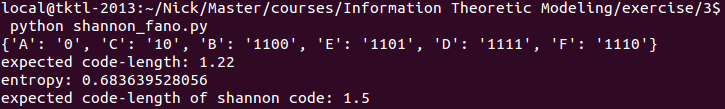
\includegraphics[width=\textwidth,keepaspectratio]{1.png}
  \centerline{Figure 1: Shannon-Fano code, applied to simple source of A to F}
\end{minipage}

\section{Problem 3}

I just use Chapter I of \emph{Alice in Wonderland} as the text for estimating the symbol occurrence probabilities. Please see the source text in \emph{alice\_preprocess} and source code in \emph{shannon\_fano2.py}. 

Based on the result of the program, the expected code-length is \textbf{4.116}, the entropy is \textbf{4.058} and the expected code-length of the Shannon code is \textbf{4.563}.

I also use huffman coding to encode the same text for comparison. The source code is in \emph{huffman2.py}, and its expected code-length is \textbf{4.105}. Figure 2 and figure 3 show the running result of Shannon-Fano code and Huffman code, respectively.

\vspace{5mm}
\begin{minipage}{0.9\textwidth}
  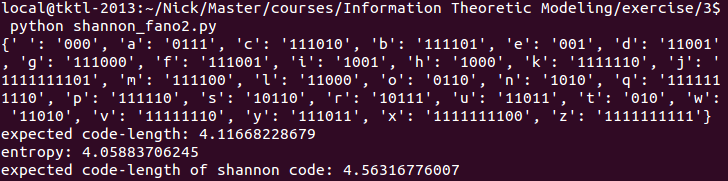
\includegraphics[width=\textwidth,keepaspectratio]{2.png}
  \centerline{Figure 2: Shannon-Fano code, applied to Chapter I of \emph{Alice in Wonderland}}
\end{minipage}

\vspace{5mm}
\begin{minipage}{0.9\textwidth}
  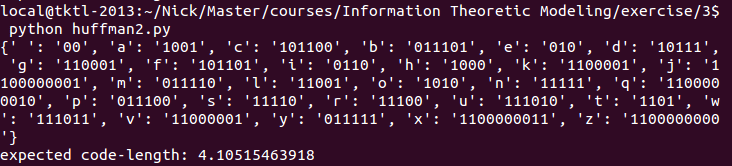
\includegraphics[width=\textwidth,keepaspectratio]{3.png}
  \centerline{Figure 3: Huffman code, applied to Chapter I of \emph{Alice in Wonderland}}
\end{minipage}

\section{Problem 4}

\subsection*{(a)}

Please see source code of Huffman code in \emph{huffman.py}. Figure 4 shows its running result.

\vspace{5mm}
\begin{minipage}{0.9\textwidth}
  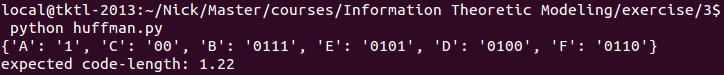
\includegraphics[width=\textwidth,keepaspectratio]{4.png}
  \centerline{Figure 4: Huffman code, applied to simple source of A to F}
\end{minipage}

\subsection*{(b)}

Such a case can be that source code only consists $A$ and $B$. $A$ has probability of \textbf{0.0001} and $B$ has probability of \textbf{0.9999}. Since probability of $A$ is quite small, so that $\lceil{log_2 1/p_i}\rceil$ will be large. But for Huffman code, the code-length of both $A$ and $B$ is one.

\subsection*{(c)}

\subsubsection*{i.}

Fewest occurrences of symbol $e$ is \emph{3} to keep the Huffman tree still maximally unbalanced. The number for $f$ is \emph{5}, for $g$ is \emph{8} and for $h$ is \emph{13}. So the sequence is $[1, 1, 1, 2, 3, 5, 8, 13, 21, 34...]$ for symbol $a$ to $j$. It is Fibonacci sequence excluding the first number.

\subsubsection*{ii.}

The probability of $a$ depends on the value of $m$. Table 1 shows the probability of $a$ depending on $m$.

\begin{table}[h]
\centering
\begin{tabular}{|c | c c c c c c c c|}
\hline
$m$	&1	&2	&3	&4  &5  &6  &7  &8\\
\hline
$p(a)$	&1  &1/2  &1/3  &1/5  &1/8  &1/13  &1/21  &1/37\\
\hline
\end{tabular}
\caption{Probability of $a$ depending on $m$}
\end{table}



\subsubsection*{iii.}

Table 2 shows the depth of the tree depending on the value of $m$.

\begin{table}[h]
\centering
\begin{tabular}{|c | c c c c c c c c|}
\hline
$m$	&1	&2	&3	&4  &5  &6  &7  &8\\
\hline
$depth$	&0  &1  &2  &3  &4  &5  &6  &7\\
\hline
\end{tabular}
\caption{Depth of the tree depending on $m$}
\end{table}

\subsubsection*{iv.}

Since the probability of $a$ has been calculated in \textbf{ii}, the Shannon codeword length can be computed using$\lceil{log 1/p(a)}\rceil$. Table 3 shows the comparison of Shannon codeword length and Huffman code.

\begin{table}[h]
\centering
\begin{tabular}{|c | c c c c c c c c|}
\hline
$m$	&1	&2	&3	&4  &5  &6  &7  &8\\
\hline
\emph{Huffman code}  &0	&1	&2	&3	&4  &5  &6  &7\\
\hline
\emph{Shannon codeword length}	&0  &1  &2  &3  &3  &4  &5  &6\\
\hline
\end{tabular}
\caption{Comparison of Huffman code and Shannon codeword length for symbol $a$.}
\end{table}


\section{Problem 5}

Firstly, we should transform the real number parameter $p$ to binary representations. We can achieve this by encoding the symbols of 0 to 9 using prefix(-free) code. Now set the parameter $p$ as some float number $0.p_1p_2p_3...$, and the potentially infinite sequence of fair coin flips as $0.z_1z_2z_3...$ in which $p_i$ and $z_i$ are binaries. To simulate the generation of $Pr[x=0]=p$, we can run a test from the first binary of $p_i$ and $z_i$. If $z_i = p_i$, then continue test. Else if $z_i < p_i$, return \textbf{0} as the simulation result. Otherwise, return \textbf{1} as the result. This is because $p$ can be seen as following the uniform distribution, thus the probability that the $z_i$ string smaller than $p_i$ string is $p$. Thus, we can get $0$ at the probability of $p$.

The probability of only using one flip is $1/2$, and the probability of using two flips is $(1/2)^2$, and so on. So the expected number of flips is:

\begin{equation*}
\begin{split}
S_{n\rightarrow+\infty} &= 1\times1/2 + 2\times(1/2)^2 + 3\times(1/2)^3 + ... +n\times(1/2)^n\\
& =2\\
\end{split}
\end{equation*}

\end{document}